\chapter{Ramsey Theory}

Before we can get started we will need some basic notions from graph theory.
\begin{definition}
	Let $G = (V, E)$ be a graph, $G$ is called \textit{complete} if $v, u \in V$ such that $v \neq u$ implies $\left\{v, u\right\} \in E$. A \textit{subgraph} of $G$ is a graph $G' = (V', E')$ such that $V' \subseteq V$ and $E' \subseteq E$. Finally a complete subgraph is called a \textit{clique}.
\end{definition}
We often denote a complete graph with $n$ vertices as $K_n$.


\begin{theorem}[Generalized Pigeonhole Principle]\label{thm:gpp}
	Let $A$ be a set such that $\abs{A} > m \cdot r$ if $A = \bigcup_{i = 1}^{r} A_i$, then there exists a $A_j$ such that $\abs{A_j} > m$.
\end{theorem}
\begin{proof}
	Assume for the sake of contradiction that $\abs{A_j} < m$ for $j = 1, 2, \ldots, r$, then:
	\begin{equation*}
		\abs{A} \leq \sum_{j = 1}^r \abs{A_i} < r \cdot m
	\end{equation*}
	clearly a contradiction.
\end{proof}

\begin{definition}
	Let $A$ be a set, a \textit{$r$-coloring} on $A$ is a function $\chi: A \to C$ where $C$ is the set of \textit{colors} and $\abs{C} = r$. The subset $A' \subseteq A$ is called \textit{monochromatic} if $\chi(a) = c$ for all $a \in A$.
\end{definition}
\begin{remark}
	The concrete choice of color set $C$, in our $r$-coloring $\chi: A \to C$, is not really a concern, since given any bijection $\phi$ between $C$ and another color set $C'$ one would obtain a new $r$-coloring $\chi' = \phi \circ \chi$.
	Hence for the sake of simplicity we pick $C = [r]$, unless $r = 2$ or $r = 3$ in which cases we usually let $C = \left\{red, blue\right\}$ or $C = \left\{red, blue, green\right\}$ respectively. Additionally we note that an $r$-coloring $\chi$ on $A$, can be thought of as an partitioning of $A$ into the sets $A_i = \left\{a \in A | \chi(a) = i\right\}$.
\end{remark}

We will primarily be interested in the case where $A$ is the set of edges $E$ of the complete graph $K_n$, in which case we will refer to $\chi$ as an edge coloring on $K_n$.

\begin{definition}
	Let $n$ be a positive natural number we will write $n \to (\ell_1, \ell_2, \ldots, \ell_{r})$ if for every $r$-edge coloring $\chi: E_{n} \to \left\{c_1, c_2, \ldots, c_{r}\right\}$ on $K_n$, there exists an $i \in \left\{1, 2, \ldots, r\right\}$ such that $\chi$ emits a $c_{i}$-monochromatic clique of order $k_{i}$.
\end{definition}
\begin{remark}
	Clearly $k_i \leq k_i'$ and $n \to (k_1, k_2, \ldots, k_{r})$ implies that $n \to (k_1', k_2', \ldots, k_{r}')$
\end{remark}

\begin{theorem}[Ramsey's Theorem]\label{thm:ramsey_two_colors}
	Let $\ell_1, \ell_2 \geq 2$, then there exists a non-zero $n \in \mathbb{N}$ such that $n \to (\ell_1, \ell_2)$.
\end{theorem}
\begin{proof}
	Clearly $\ell_1 \to (\ell_1, 2)$ and $\ell_2 \to (2, \ell_2)$ (after all either $K_{\ell_{i}}$ is monochromatic or there exist a monochromatic clique of order $2$). We will proceed using induction on $\ell_1 + \ell_{2}$, we may assume that $\ell_1 + \ell_2 \geq 6$, with $\ell_1, \ell_2 \geq 3$.
	Additionally by our induction hypothesis we may assume the existence of non-zero $n_1, n_2 \in \mathbb{N}$ such that $n_1 \to (\ell_1, \ell_2 - 1)$ and $n_2 \to (\ell_1 - 1, \ell_2)$. Next let $n := n_1 + n_2$ we will show that $n \to (\ell_1, \ell_2)$. Fix an arbitrary $2$-edge coloring $\chi$ on $K_n$ and let $v$ be a vertex in $K_n$, then $v$ is adjcent to $n - 1$ other vertices in $K_{n}$, hence:
	\begin{equation*}
		n_1 + n_2 - 1 = n - 1 = \abs{N_{\chi}(v; 1)} + \abs{N_{\chi}(v; 2)}
	\end{equation*}
	meaning either $\abs{N_{\chi}(v; 1)} \geq n_2$ or $\abs{N_{\chi}(v; 2)} \geq n_1$. Without loss of generality assume that the second inequality holds, namely $\abs{N_{\chi}(v; 2)} \geq n_1$. By our inductive hypothesis, the complete graph $G = (N_{\chi}(v; 2), N_{\chi}(v; 2) \times N_{\chi}(v; 2))$ contains either a $1$-monochromatic clique of order $\ell_{1}$ (in which case we are done) or a $2$-monochromatic clique of order $\ell_{2} - 1$, in which case we note that $v$ is connected to the vertices in $N_{\chi}(v; 2)$ via edges that $\chi$ assigns the color $2$, hence complete graph on the vertex set $N_{\chi}(v; 2) \cup \left\{v\right\}$ forms a $2$-monochromatic clique of order $\ell_{2}$.
\end{proof}

\begin{corollary}\label{cor:ramsey_for_arbitarily_many_colors}
	Let $\ell_1, \ell_2, \ldots, \ell_r \geq 2$, then there exists a non-zero $n \in \mathbb{N}$ such that $n \to (\ell_1, \ell_2, \ldots, \ell_{r})$.
\end{corollary}

\begin{proof}
	We proceed using induction on $r$, the base case $r = 2$ is proven in Theorem \ref{thm:ramsey_two_colors}.
	Next assume that the theorem holds for $r - 1$. From Theorem \ref{thm:ramsey_two_colors}, it follows that there exists a $\ell \in \mathbb{N}_{> 0}$ such that $\ell \to (\ell_{r - 1}, \ell_{r})$.
	By our induction hypothesis we may find a $n \in \mathbb{N}_{> 0}$ for which it holds that:
	\begin{equation*}
		n \to (\ell_1, \ell_2, \ldots, \ell_{r - 2}, \ell)
	\end{equation*}
	Now given any $r$-edge coloring $\chi$ on $K_n$ we may obtain a $r - 1$-edge coloring $\chi'$ on $K_n$ by defining:
	\begin{equation*}
		\chi'(e) = \begin{cases} \chi(e) & \text{ if } \chi(e) < r - 1 \\ r - 1 & \text{ otherwise } \end{cases}
	\end{equation*}
	Hence $\chi'$ must either emit a $i$-monochromatic clique of order $\ell_i$, for some $i \in \left\{1, 2, \ldots, r - 2\right\}$ (in which case we are done) or a $(r - 1)$-monochromatic clique of order $\ell$. Let $K_\ell$ be this monochromatic clique, then $\chi$ associates every edge in $G$ with either $r - 1$ or $r$. However $\ell$ was chosen so that $\ell \to (\ell_{r - 1}, \ell_r)$, hence $G$ must contain either a $(r - 1)$-monochromatic clique of order $\ell_{r - 1}$ or a $r$-monochromatic clique of order $\ell_{r}$.
\end{proof}

\begin{definition}
	The \textit{Ramsey number} $R(k_1, k_2, \ldots, k_{r})$, is the minimal $n \in \mathbb{N} \setminus \left\{0\right\}$ such that $n \to (k_1, k_2, \ldots, k_{r})$, additionally we let $R(k; r)$ denote $R(k_1, k_2, \ldots, k_{r})$, with $k_1 = k_2 = \cdots = k_r = k$.
\end{definition}
Generally direct computation of Ramsey numbers are extremely difficult,




\begin{example}\label{exmp:R3_3}
	In this example we will show that $R(3, 3) = 6$, we start by showing that $R(3, 3) \leq 6$. Consider the edge coloring $\chi: E(K_{6}) \to \left\{red, blue\right\}$ on $K_6$ and let $v$ be a vertex in $K_6$, then $v$ has $5$ adjacent neighbours, by the generalized pigeonhole principle, Theorem \ref{thm:gpp}, there is a color $c$ (either $red$ or $blue$) such that $\abs{N_{\chi}(v; c)} \geq 3$.

	Without loss of generality we may assume that $c = red$. Next take pairwise distinct $v_1, v_2, v_3 \in N_{\chi}(v; red)$, then we must have $\chi(v_{i}, v_{j}) = blue$ for pairwise distinct $i, j \in [3]$, since we otherwise would have that $K_{6} |_{\left\{v, v_i, v_j\right\}}$ would form a $red$-monochromatic clique of order $3$. However this in turn means that $\chi(v_i, v_j) = blue$ for all pairwise distinct $i, j \in [3]$, hence $K_6 |_{\left\{v_1, v_2, v_3\right\}}$ forms a $blue$-monochromatic clique of order $3$.

    On the other hand it is easy to construct a $2$-edge coloring on $K_5$ which emits no monochromatic subclique of order $3$, see for instance the graph in Figure \ref{fig:K5_counter_example}.
    \begin{figure}[H]
  \centering
  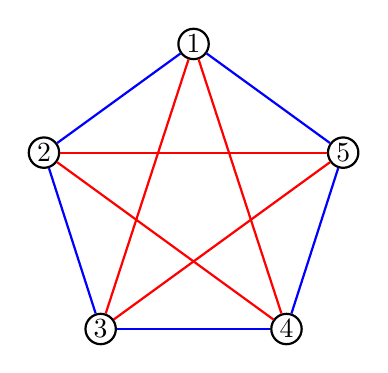
\begin{tikzpicture}
    \tikzset{punkt/.style={circle, thick, draw=black, minimum width=0.2cm,inner sep=1}}
    \node[punkt] at (0.0, 2.0) (a) {$1$};
    \node[punkt] at (-1.9, 0.62) (b) {$2$};
    \node[punkt] at (-1.18, -1.62) (c) {$3$};
    \node[punkt] at (1.18, -1.62) (d) {$4$};
    \node[punkt] at (1.9, 0.62) (e) {$5$};
    %\draw (0,0) circle [radius=2];

    % Blue edges
    \draw [thick, draw=blue] (a) -- (b);
    \draw [thick, draw=blue] (b) -- (c);
    \draw [thick, draw=blue] (c) -- (d);
    \draw [thick, draw=blue] (d) -- (e);
    \draw [thick, draw=blue] (e) -- (a);

    % Red edges
    \draw [thick, draw=red] (a) -- (c);
    \draw [thick, draw=red] (a) -- (d);
    \draw [thick, draw=red] (b) -- (d);
    \draw [thick, draw=red] (b) -- (e);
    \draw [thick, draw=red] (c) -- (e);
  \end{tikzpicture}
  \caption{A 2-edge coloring on $K_{5}$ that emits no monochromatic subclique of order $3$.}
  \label{fig:K5_counter_example}
\end{figure}
Finally since $R(3, 3) > 5$ and $R(3, 3) \leq 6$, we obtain that $R(3, 3) = 6$.
\end{example}

\section{Schur's Theorem}
In this chapter, we will answer the question: ``Given a $r$-coloring on $\mathbb{N}^+$, does there always exist a monochromatic set $\left\{x_1, x_2, \ldots, x_{k}, \sum_{i = 0}^k x_i\right\} \subseteq \mathbb{N}^+$''. To get a better intuition for the problem, consider the case where $r = 3$ and $k = 2$ and $\mathbb{N}^+$ is colored by:
\begin{equation*}
	\chi(n) = \begin{cases} red   & \text{ if } n \equiv 0 \mod 3  \\
              blue  & \text{ if }  n \equiv 1 \mod 3 \\
              green & \text{ otherwise }
	\end{cases}
\end{equation*}
A visual representation of $\chi$ would be: $\textcolor{blue}{1}, \textcolor{green}{2}, \textcolor{red}{3}, \textcolor{blue}{4}, \textcolor{green}{5}, \textcolor{red}{6}, \ldots$ meaning one example of a $red$-monochromatic subset of the form $\left\{x, y, x + y\right\}$, under $\chi$, would be $x = y = 3$, notice that we do not require $x$ and $y$ to be distinct.

Next we will show that the proposition mentioned in the begining of the section does indeed hold.
\begin{theorem}[Schur's Theorem]\label{thm:schur}
	Let $r, k$ be positive integers, then there exists a least positive integer $S(r, k)$ such that any $r$-coloring $\chi: [1, S(r, k)] \to C$ there exists a monochromatic subset of $[1, S(r, k)]$ of the form $\left\{x_1, x_2, \ldots, x_{k}, \sum_{i = 1}^k x_i\right\}$.
\end{theorem}
\begin{proof}
	We will show that any $r$-coloring $\chi$ of $[1, R(k + 1; r)]$ emits a monochromatic subset of the form $\left\{x_1, x_2, \ldots, x_{k}, \sum_{i = 1}^k x_i\right\}$.

	Let $G$ be the complete graph with vertex set $[1, R(k + 1; r) + 1]$. We will define an $r$-edge coloring on $G$ by defining $\chi': E(G) \to C$ as $\chi'(\left\{a, b\right\}) := \chi(\abs{a - b})$, by the definition of $R(k + 1; r)$, the edge coloring $\chi'$ must emit a monochromatic clique $G'$ of order $k + 1$. Next if we order the verticies $v_1, v_2, \ldots v_{k + 1}$ in $G'$ in increasing order, meaning $v_1 < v_2 < \ldots < v_{k + 1}$.
	Then, since $G'$ is monochromatic, we see that
	\begin{equation*}
		\chi(v_i - v_j) = \chi'(\{v_i, v_j\}) = \chi'(\{v_{i'}, v_{j'} \}) = \chi(v_{i'} - v_{j'})
	\end{equation*}
	for all $i > j$ and $i' > j'$, since the verticies are ordered in increasing order. The rest follows by setting $x_j := v_{j + 1} - v_{j}$.
\end{proof}
Let $\chi_{0}: \mathbb{N}^+ \to C$ be an $r$-coloring then, by Schur's Theorem \ref{thm:schur}, there exists a monochromatic subset $A_0 := \left\{x_1, x_2, \ldots, x_{k}, \sum_{i = 1}^k x_i\right\}$ of $[1, S(r, k)]$. Next we may define a new coloring $\chi_1$, which colors every element in $\mathbb{N}^+ \setminus A_{0}$ the same color as $\chi_{0}$, but each element in $A_{0}$ a distinct new color, hence $\chi_1$ is at most a $(r + k + 1)$-coloring, which similarly admits a monochromatic subset $A_1 := \left\{y_1, y_2, \ldots, y_{k}, \sum_{i = 1}^k y_{i}\right\}$ of $[1, S(r + k + 1, k)]$. Additionally we note that $\chi_1(n) = \chi_0(n)$ for each $n \in A_1$ since each element in $A_0$ is colored a new distinct color, by $\chi_{1}$. Hence $A_1$ is also monochromatic under $\chi_0$. Repeating this argument we obtain the following corollary:
\begin{corollary}
	Let $r, k$ be positive integers, any $r$-coloring $\chi: \mathbb{N}^{+} \to \left\{c_1, c_2, \ldots, c_{r}\right\}$ emits infinitely many monochromatic subsets $\mathbb{N}^{+}$ of the form $\left\{x_1, x_2, \ldots, x_{k}, \sum_{i = 1}^k x_i\right\}$.
\end{corollary}


Next we show that statement of Fermats last theorem: ``The equation $x^n + y^n = z^n$, with $n \geq 2$, has no solution $x, y, z \in \mathbb{Z}$, such that $xyz \neq 0$.'' is false if we instead require that $x, y, z$ are elements in some specific family of finite fields.

\begin{theorem}
	Let $n \geq 1$, then there exists a prime $p$ such that for all primes $q \geq p$, the equation $x^n + y^n = z^{n}$ has a solution $x, y, z \in \mathbb{F}_{q}$ with $xyz \neq 0$.
\end{theorem}
\begin{proof}
	Let $q > S(n, 2)$ be a prime, we will consider the multiplicative group $\mathbb{F}_q^{*}$, and the subgroup $G = \left\{x^n \mid x \in \mathbb{F}_p\right\}$.

	Hence there exists $a_1, a_2, \ldots a_k \in \mathbb{F}_q^{*}$ such that $\mathbb{F}_q^{*} = \bigcup_{i = 1}^k a_i G$ with $k = \frac{n}{\gcd(n, p - 1)}$ \textcolor{red}{\textbf{TODO}}. Since $\abs{\mathbb{F}_q^{*}} = \abs{\mathbb{F}_q^{*} / S}\abs{S}$ (lagrange index theorem) and

	Next, we define a $k$-coloring $\chi: \mathbb{F}_q^* \to [k]$ by $\chi(y) = j$ if and only if $y \in a_j G$. Now since $k \leq n$ and $p - 1 \geq S(n, 2)$, there exists a monochromatic triple $\left\{x, y, z\right\} \subseteq \mathbb{F}_q^{*}$ such that $x + y = z$, by Theorem \ref{thm:schur}. Meaning there exists an index $j \in [k]$ such that $a_{j}x^{n}, a_jy^{n}, a_{j}z^{n} \in a_jS$ with $a_{j}x^{n} + a_{j}y^{n} = a_jz^{n}$, the rest follows by multiplying by $a_{j}^{-1}$.
\end{proof}

